\chapter{Gravitational-wave Merger Forecasting: Scenarios for the Early Detection and Localization of Compact-binary Mergers with Ground-based Observatories}\label{ch:forecasting}
\chaptermark{Gravitational-wave Merger Forecasting}
This chapter summarizes the work published as \cite{Nitz:2020vym}. It discusses a classical low-latency search for pre-merger detection of \acrshort{bns} systems. It is covered in this thesis, as machine learning is often stated to be a tool to decrease latency. Having a reference point of existing algorithms that are capable of pre-merger detection is important to determine research areas where machine learning algorithms may be of practical use.

\section{Introduction}
GW170817~\cite{LIGOScientific:2017vwq} was the first detected \acrshort{gw} event emitted by a \acrshort{bns} merger. It was accompanied by an \acrshort{em} counterpart observed in multiple frequency bands~\cite{LIGOScientific:2017ync}. The earliest \acrshort{em} signal was a gamma ray burst observed by Fermi-GBM and INTEGRAL~\cite{Goldstein:2017mmi, Savchenko:2017ffs, Monitor:2017mdv} about \SI{1.7}{\second} after the \acrshort{gw} merger. The first optical observations began only about $11$ hours after the merger~\cite{Coulter:2017wya}. These \acrshort{em} observations provided new insight into the nuclear equation of state~\cite{LIGOScientific:2018hze, LIGOScientific:2018cki, Radice:2017lry, Kiuchi:2019lls, Capano:2019eae, LIGOScientific:2019eut}, the Hubble constant~\cite{Guidorzi:2017ogy, Hotokezaka:2018dfi, LIGOScientific:2018gmd}, the phenomenon of kilonova (see ~\cite{Metzger:2019zeh} and references therein), and the central engine of short gamma-ray bursts~\cite{Murguia-Berthier:2020tfs, Wu:2019rla, Lazzati:2020vbo, Nitz:2020vym}.

If early observations of the optical band would have been available, different kilonova emission models could have been differentiated~\cite{Arcavi:2018mzm}. It is also hypothesisized that pre-merger \acrshort{em} emissions exist~\cite{Hansen:2000am, Troja:2010zm, Tsang:2011ad, Metzger:2016mqu, Wang:2016dgs, Wada:2020kha}, which could be constrained by pre-merger observations. However, early or even pre-merger \acrshort{em} observation of \acrshort{cbc} mergers are constrained by two factors: The latency between \acrshort{gw} signal detection and telescopes being alerted, as well as the ability of \acrshort{em} instruments being able to cover the sky area where the source is estimated to be located.

This study assesses the possibility of generating pre-merger alerts for different eras of detectors and quantifies the localization error associated with them. By providing pre-merger alerts, the latency is automatically reduced. Quantifying the localization error allows for \acrshort{em} observation strategies to be optimized and coordinated. To do so, the evolution of the pre-merger alert capabilities of ground based detectors over the next $\mathcal{O}(10)$ years are evaluated. Additionally, the capabilities of the current low-latency PyCBC Live~\cite{Nitz:2018rgo, DalCanton:2020vpm} analysis to generate early warnings is tested.

\section{Methods}
Our study covers the five current and planned ground based \acrshort{gw} observatories of the coming decade \acrshort{ligo}-Hanford (H), \acrshort{ligo}-Livingston (L)~\cite{LIGOScientific:2014pky}, \acrshort{ligo}-India (I)~\cite{Iyer:2011aaa}, Virgo (V)~\cite{VIRGO:2014yos}, and KAGRA (K)~\cite{KAGRA:2018plz}. For this network of detectors, we consider three different eras: ``Design'', ``A+'', and ``Voyager''. The ``Design'' era expects the four detectors \acrshort{ligo}-Hanford, \acrshort{ligo}-Livingston, Virgo, and KAGRA to be operational at their 2021-2022 design sensitivity~\cite{KAGRA:2013rdx}. Starting with the ``A+'' era, we expect \acrshort{ligo}-India to be operational and matching the sensitivity of both \acrshort{ligo}-Hanford and \acrshort{ligo}-Livingston. We use the design \acrshort{psd} of the planned upgrades to the \acrshort{ligo} instruments from 2024-2026 for the three \acrshort{ligo} detectors~\cite{Barsotti:2018aaa}. For Virgo and KAGRA we conservatively assume that their sensitivity will not improve beyond their ``Design'' era. The ``Voyager'' era assumes the \acrshort{psd} of the three \acrshort{ligo} detectors to match the ``Voyager'' plans~\cite{LIGOScientific:2017aaa}. A follow-up study covered the third generation detectors \acrshort{et} and \acrshort{cw}~\cite{Nitz:2021pbr}.

To assess the capability of pre-merger detection in the different configurations discussed in \cite{Nitz:2020vym}, we simulated a population of $\mathcal{O}(10^5)$ \acrshort{bns} mergers. This population is distributed uniformly in volume and isotropically in sky location and binary orientation. The masses are chosen to be a reference binary with \SI[parse-numbers=false]{1.4-1.4}{M_\odot}, but the results can be generalized to arbitrary masses (see Section 4 in \cite{Nitz:2020vym}). The signals are subsequently injected into simulated, Gaussian noise, colored by the \acrshort{psd} of different detectors and eras.

We pursue two different criteria for signal detection. To gauge the general capability of pre-merger detection, our first method assumes the detection of a signal if the combined optimal network \acrshort{snr} $> 10$. This choice is consistent with the threshold for confidently detected mergers in~\cite{LIGOScientific:2018mvr, Nitz:2020oeq}. To determine the pre-merger detection capabilities, we calculate the network \acrshort{snr} as a function of time before merger. Once the network \acrshort{snr} exceeds the threshold, it is counted as detected and we generate a posterior of the sky location using Baystar~\cite{Singer:2015ema} for every time step. The second method involves a full search using PyCBC Live in a low-latency configuration at a \acrshort{far} of $1$ per year. To adapt it to pre-merger detection, the template bank is a combination of several template banks using different pre-merger truncation times. The truncation of the different banks are chosen such that they cover $5\%$ increments of the total expected \acrshort{snr}. This second analysis allows us to test how capable existing analysis methods are at pre-merger detection. Sky localization is again performed using Baystar~\cite{Singer:2015ema}.

\section{Results}
The core results of the study are given in Figures \ref{fig:res_design} to \ref{fig:res_voyager}. They show the search sensitivity, localization error accuracy, and detection rate estimates as functions of time of detection before merger. The two columns compare the network of currently operational detectors with the planned detector network for each era. The times on the horizontal axis do not include the latency of the analysis or any other processing. They merely reflect the upper frequency cutoff at which the two analysis methods can detect them.
\begin{figure}
	\centering
	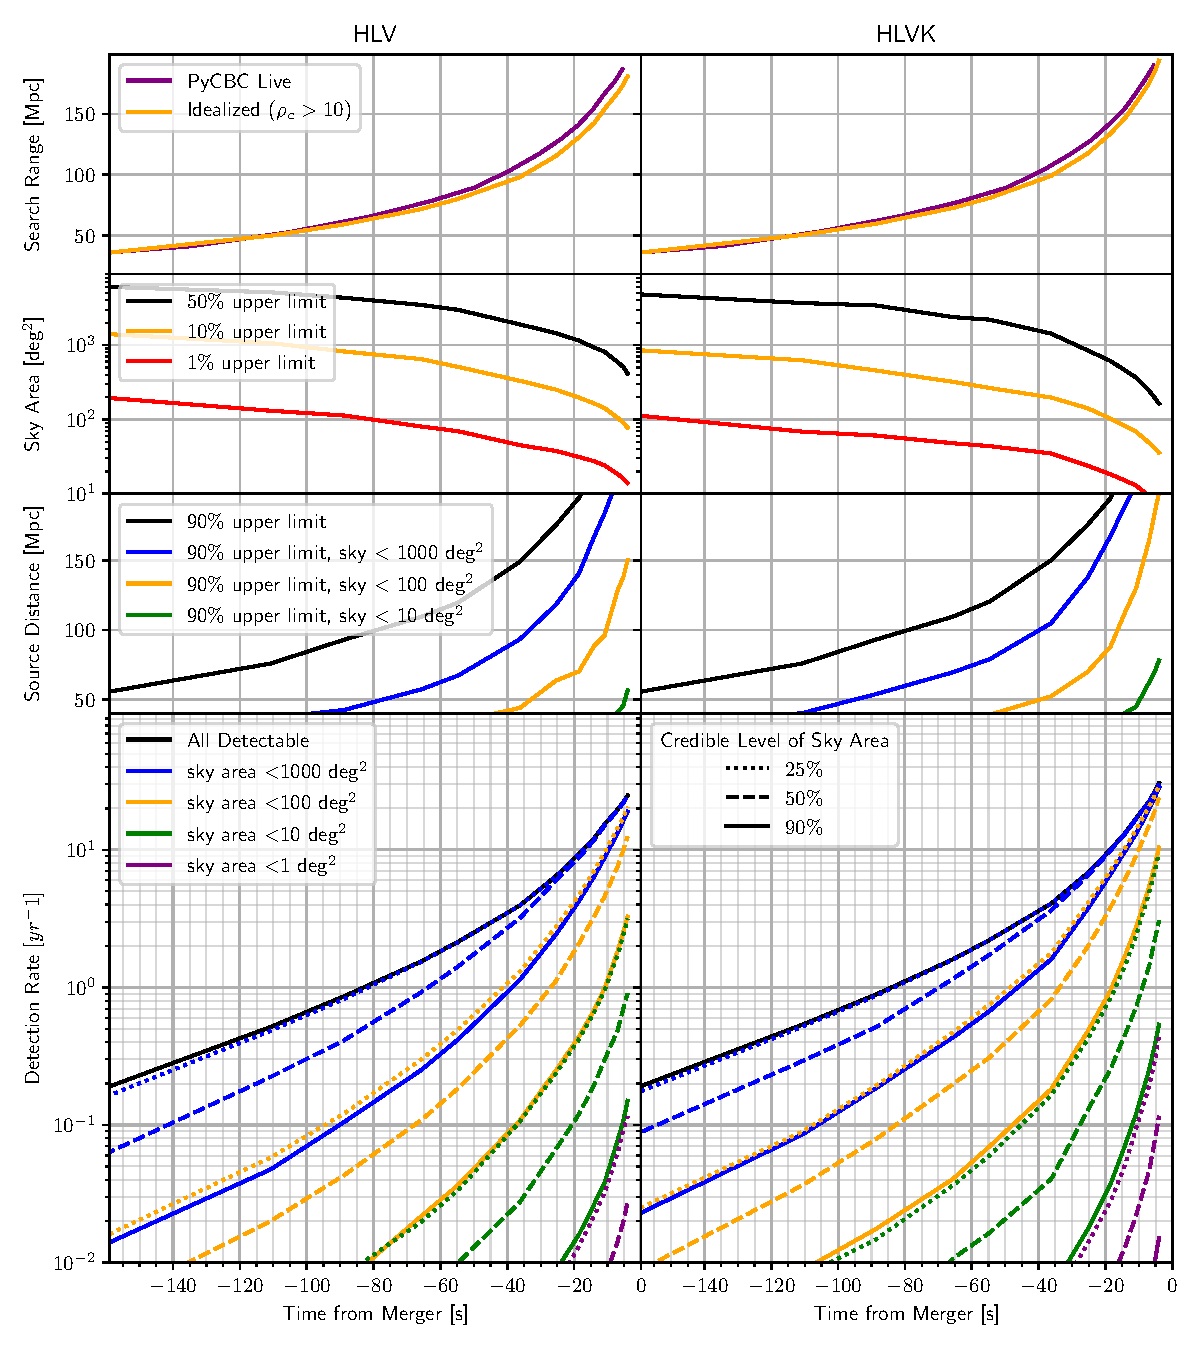
\includegraphics[width=\textwidth]{chapters/forecasting/images/design.pdf}
	\caption[``Design'' era detection ranges, localizations, distances, and merger rates]{``Design'' era (2021-2022) detection and localization for the HLV network (left) and the full gravitational-wave detector network (right) as a function of time before merger for a fiducial 1.4-1.4$M_\odot$ BNS merger. (Top) The sky-averaged detection range for the idealized search and PyCBC Live operating at a false alarm rate of once per year. (Middle) The upper limit on the localization sky area and source distance, respectively, for detectable sources. Sky areas are quoted at the 90$\%$ credible level. (Bottom) The detection rate of all sources (black) and those that also have a sky localization less than 1000 deg$^2$ (blue), 100 deg$^2$ (orange), 10 deg$^2$ (green), or 1 deg$^2$ at a 90$\%$ (solid), 50$\%$ (dashed), and 25$\%$ credible level (dotted). Figure and caption are taken from \cite{Nitz:2020vym}.}\label{fig:res_design}
\end{figure}
\begin{figure}
	\centering
	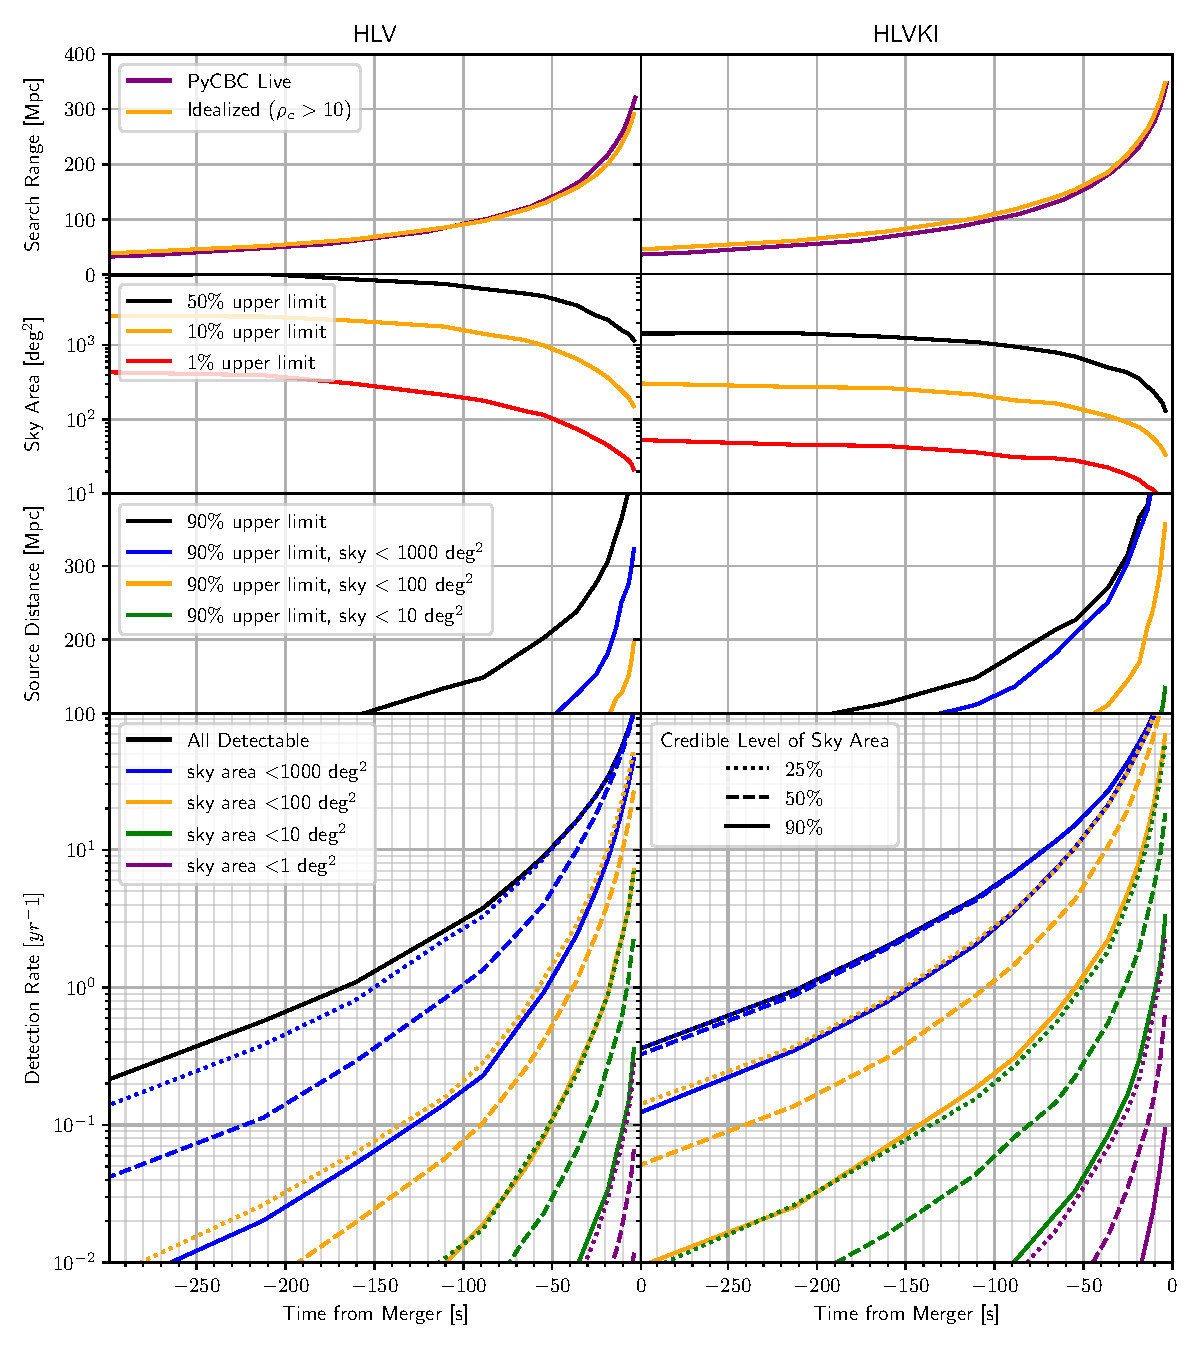
\includegraphics[width=\textwidth]{chapters/forecasting/images/aplus.pdf}
	\caption[``A+'' era detection ranges, localizations, distances, and merger rates]{``A+'' era (2024-2026)  detection and localization for the HLV network (left) and the full gravitational-wave detector network (right) as a function of time before merger for a fiducial 1.4-1.4$M_\odot$ BNS merger. (Top) The sky-averaged detection range for the idealized search and PyCBC Live operating at a false alarm rate of once per year. (Middle) The upper limit on the localization sky area and source distance, respectively, for detectable sources. Sky areas are quoted at the 90$\%$ credible level. (Bottom) The detection rate of all sources (black) and those that also have a sky localization less than 1000 deg$^2$ (blue), 100 deg$^2$ (orange), 10 deg$^2$ (green), or 1 deg$^2$ at a 90$\%$ (solid), 50$\%$ (dashed), and 25$\%$ credible level (dotted). Figure and caption are taken from \cite{Nitz:2020vym}.}\label{fig:res_aplus}
\end{figure}
\begin{figure}
	\centering
	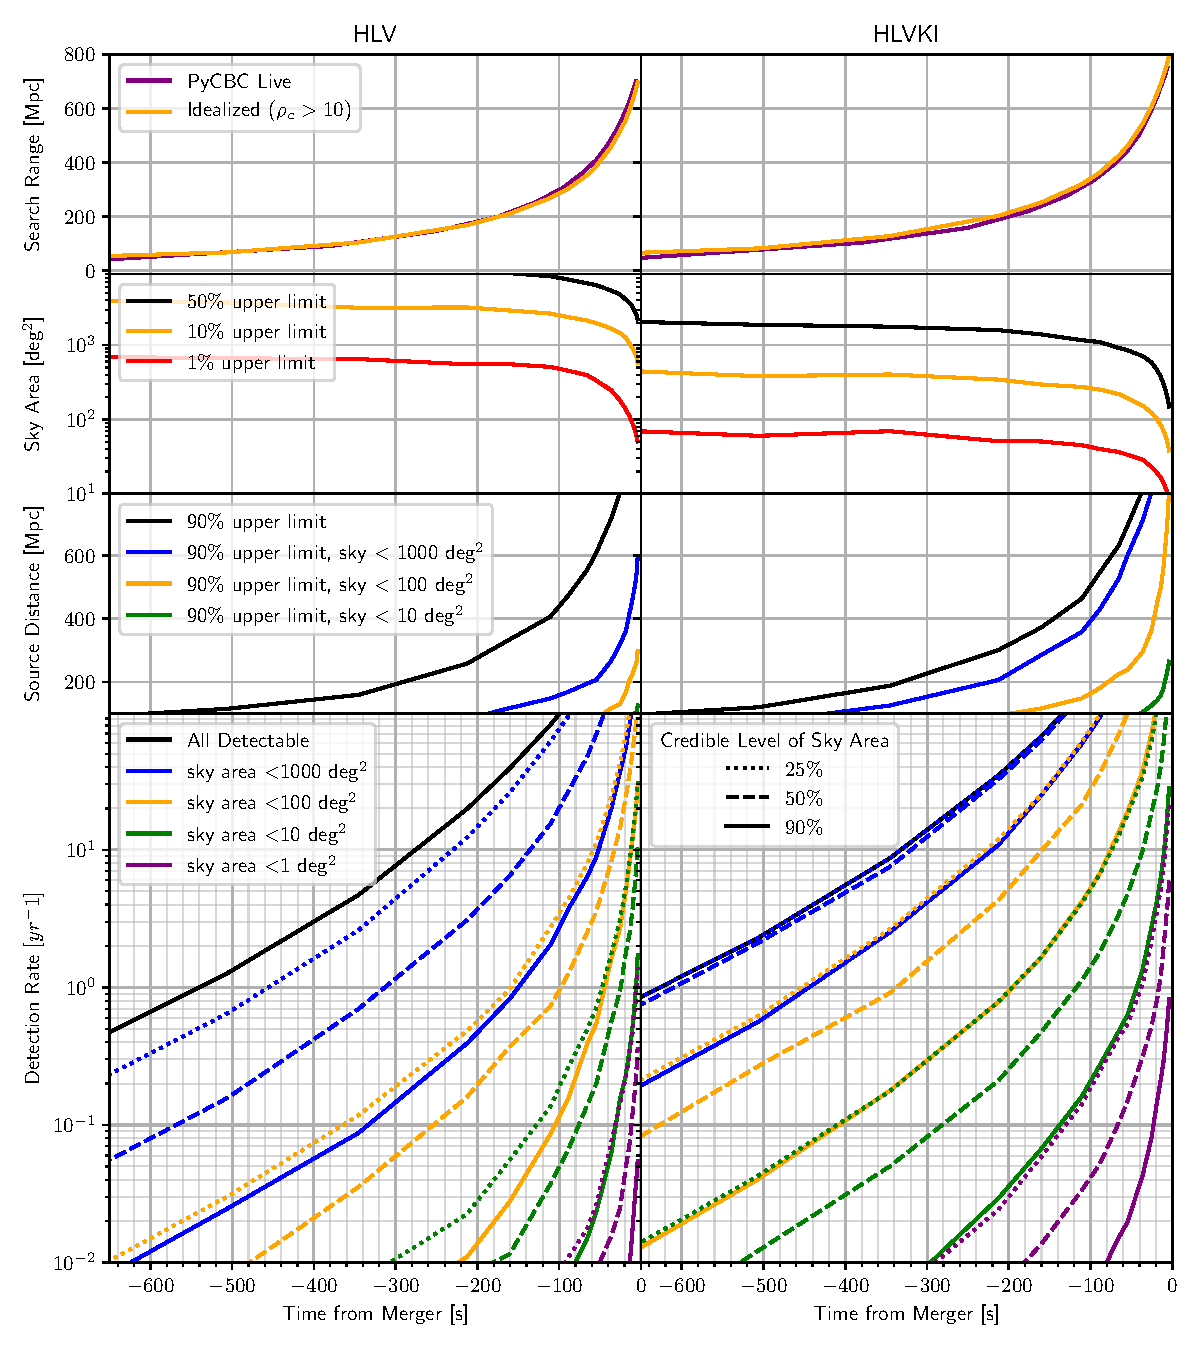
\includegraphics[width=\textwidth]{chapters/forecasting/images/voyager.pdf}
	\caption[``Voyager'' era detection ranges, localizations, distances, and merger rates]{``Voyager'' era (late 2020's)  detection and localization for the HLV network (left) and the full gravitational-wave detector network (right) as a function of time before merger for a fiducial 1.4-1.4$M_\odot$ BNS merger. (Top) The sky-averaged detection range for the idealized search and PyCBC Live operating at a false alarm rate of once per year. (Middle) The upper limit on the localization sky area and source distance, respectively, for detectable sources. Sky areas are quoted at the 90$\%$ credible level. (Bottom) The detection rate of all sources (black) and those that also have a sky localization less than 1000 deg$^2$ (blue), 100 deg$^2$ (orange), 10 deg$^2$ (green), or 1 deg$^2$ at a 90$\%$ (solid), 50$\%$ (dashed), and 25$\%$ credible level (dotted). Figure and caption are taken from \cite{Nitz:2020vym}.}\label{fig:res_voyager}
\end{figure}

From the plots, we find that the PyCBC Live analysis is comparable to the idealized search and even outperforms it at a \acrshort{far} of 1 per month. This shows that current analysis methods are fully capable of pre-merger detections at the calculated rates. Assuming a merger rate density of \SI{1000}{\giga\parsec^{-3}\years^{-1}}, we find that one source per year can be expected to be detected with a $90\%$ confidence localization of $<100$~deg$^2$ and an early warning of \SI{18}{\second}, \SI{54}{\second}, and \SI{195}{\second} for the ``Design'', ``A+'', and ``Voyager'' era, respectively. If the confidence region is reduced to $50\%$, the early warning increases to \SI{34}{\second}, \SI{104}{\second}, and \SI{335}{\second}. Alternatively, the pre-merger warning can be kept constant to increase the expected number of detections to $4-6$ sources per year. This strategy would more than double the number of detected \acrshort{em} counterparts, assuming that $50\%$ of the counterparts lie outside the credible region.
\newpage

\section{Conclusions}
We have shown that for different detector network configurations in the coming decade the possible pre-warning time for a \acrshort{bns} merger may increase from $\mathcal{O}\lr{10}$ to $\mathcal{O}\lr{100}$ seconds. However, this amount of pre-warning is still insufficient for many observatories for re-pointing and tiling a $100$ deg$^2$ area~\cite{Coughlin:2019qkn}. Notable exceptions include Swift~\cite{Tohuvavohu:2020stm}, ZTF~\cite{Bellm:2018aaa, Coughlin:2019xfb}, MASTER~\cite{Kornilov:2011fi}, and CTA~\cite{CTAConsortium:2013ofs}. Observatories that are not capable of re-point and tile the sky region in the provided early warning time may still benefit by adjusting their observing configurations~\cite{James:2019xca}.

We hope that this roadmap provides grounds for the observing community to plan continued and automated observations with existing instruments, as well as further motivation to build new instruments with different observation bands. This includes concepts such as the Transient Astrophysics Probe~\cite{Camp:2019aaa}. If these hopes are met, it seems plausible that the first \acrshort{bns} detection with simultaneous observation of the prompt \acrshort{em} emissions can be made within the next decade. 
